% !TEX root = main.tex

\begin{quote}
    \em
    \vphantom{~}\llap{\adfdownleafleft\;}โจทย์ประเภท Coding
    เป็นโจทย์สไตล์ competitive programming ที่ผู้เข้าแข่งขันจะต้องทำความเข้าใจโจทย์ปัญหาเชิงคำนวณ
    แล้วเลือกโครงสร้างข้อมูลหรืออัลกอริทึมที่เหมาะสมมาแก้ปัญหาดังกล่าว\;
    ผู้เข้าแข่งขันจะต้องเขียนโปรแกรมด้วยภาษาที่ตนเองถนัดมารับ input 
    ไปประมวลผล แล้วจึง output ผลลัพธ์ที่ประมวลผลได้\;
\end{quote}

%% Setup specific blocking for centering verbatim
\newlength{\monochar}
\settowidth{\monochar}{\texttt{a}}
\newenvironment{centervrb}[1]{%
\begin{minipage}[t]{#1\monochar}
\setstretch{0.8}
}{%
\end{minipage}
}

\question{\bfseries Island Counting}

\subsection*{\sectionfont\upshape Background}

ในเกมย้อนยุคเกมหนึ่ง มีการวาดแผนที่ด้วย ASCII Art โดยประกอบไปด้วยอักขระ ASCII 
ที่เรียงตัวกันเป็นสี่เหลี่ยมผืนผ้าจำนวน $R$ แถว แถวละ $C$ ตัว

อักขระแต่ละตัวจะแทนช่อง 1 ช่องและมีค่าได้ 2 แบบ ได้แก่
\begin{itemize}
    \item ผืนดิน ซึ่งเราจะขอแทนด้วย `\verb|#|'
    \item ผืนน้ำ ซึ่งเราจะขอแทนด้วย `\verb|.|'
\end{itemize}

นอกจากนี้เราจะสมมติว่า รอบนอกสี่เหลี่ยมผืนผ้านี้จะ\uline{มีแต่น้ำทะเล}อันกว้างใหญ่ไพศาลและ\uline{ไม่มีผืนดิน}อยู่เลย

\bigskip\noindent
\textbf{\uline{ตัวอย่าง}}* นี่คือแผนที่ตัวอย่าง ซึ่งมีขนาด $R = {6}$ และ $C = {18}$
\begin{center}
    \vspace{0.25\baselineskip}
    \begin{centervrb}{18}
\begin{plainvrb}
................##
..#####...##......
.##...##..##...###
.#..#..#.......#..
.#....##..#.#..#.#
.######....#...#.#
\end{plainvrb}
    \end{centervrb}
    \vspace{0.25\baselineskip}
\end{center}

\subsection*{\sectionfont\upshape What is an island?}
จากแผนที่ในลักษณะข้างต้น เรานิยามภูมิประเทศทีของเกาะดังนี้%

\begin{itemize}
\item หากเราเริ่มต้นจากตำแหน่งผืนดินใด ๆ ในแผนที่ แล้วสามารถเดินทางไปยังผืนดินอื่น~ๆ 
    ข้างเคียงได้ด้วยการเดิน ขึ้น--ลง--ซ้าย--ขวา ไปเรื่อย~ๆ ได้ 
    ให้ถือว่าผืนดินที่เดินไปถึงทั้งหมดเหล่านั้นเป็นส่วนหนึ่งของเกาะเดียวกัน
\item มากไปกว่านั้น จากการเดินข้างต้น หากเราเริ่มเดินจนวกกลับมาที่ผืนดินเริ่มต้น 
    ให้ถือว่าบริเวณที่ถูกรายล้อมด้วยการเดินข้างต้นเป็นส่วนหนึ่งของเกาะเดียวกันเช่นกัน
    \begin{itemize}[before*=\small]
    \item สังเกตว่าอาจมีทะเลสาบที่ถูกรายล้อมด้วยผืนดินของเกาะเกาะหนึ่ง 
        ซึ่งผืนน้ำดังกล่าวจะถูกนับไปส่วนหนึ่งของเกาะนั้นด้วย
    \item ไม่เพียงแค่นั้น ผืนดินที่ซ้อนอยู่ภายในทะเลสาบดังกล่าว 
        ก็ยังถือว่าเป็นส่วนของเกาะภายนอกด้วย ไม่นับเป็นเกาะแยกต่างหาก
    \end{itemize}
\end{itemize}

\bigskip\noindent
\textbf{\uline{ตัวอย่าง}}* จากแผนที่ตัวอย่างเดิมข้างต้น 
เราสามารถเขียนใหม่โดยส่วนของเกาะเดียวกันเขียนด้วยตัวอักษรเดียวกันได้ดังนี้
(สังเกตได้ว่าแผนที่นี้จะมีเกาะทั้งสิ้น 8 เกาะ)
\begin{center}
    \vspace{0.25\baselineskip}
    \begin{centervrb}{18}
\begin{plainvrb}
................AA
..BBBBB...CC......
.BBBBBBB..CC...DDD
.BBBBBBB.......D..
.BBBBBBB..E.F..D.G
.BBBBBB....H...D.G
\end{plainvrb}
    \end{centervrb}
    \vspace{0.25\baselineskip}
\end{center}    

\subsection*{\sectionfont\upshape Problem Statement}

จากแผนที่ภายในเกมที่กำหนดให้ มีเกาะทั้งสิ้นกี่เกาะ?

\subsection*{\sectionfont\upshape Program Specification}

โปรแกรมที่คุณเขียนจะต้องอ่านข้อมูลจาก stardard input 
และเขียนคำตอบลง standard output โดยข้อมูลจะมีฟอร์แมตดังต่อไปนี้

\bigskip\noindent
{\sectionfont\bfseries Input Format}
\begin{itemize}[itemsep=0pt]
\item บรรทัดที่ 1: มีจำนวนเต็มสองตัว $R, C$ คั่นด้วยช่องว่าง
\item อีก $R$ บรรทัดถัดมา บรรทัดที่ $i+1$ จะมีสตริงความยาว $C$ 
    ที่ประกอบไปด้วย `\verb|.|' หรือ `\verb|#|' (ซึ่งบอกข้อมูลแถวนั้น ๆ ของแผนที่)
\begin{lstlisting}
R C
M[1,1...C]
M[2,1...C] <%\SuppressNumber\AlternateNumber{...}%>
           <%\AlternateNumber{R+1}%>
M[R,1...C] <%\ReactivateNumber%>
\end{lstlisting}
\textbf{หมายเหตุ:} ตัวแปร \verb|M| ข้างต้น คือแผนที่ซึ่งเขียนในรูปของ 1-indexed array สองมิติ
\end{itemize}

\medskip\noindent
{\sectionfont\bfseries Output Format}
\begin{itemize}
\item คำตอบประกอบด้วยจำนวนเต็มตัวเดียว ซึ่งระบุจำนวนเกาะในแผนที่ที่กำหนดให้
\end{itemize}

\newpage
\subsection*{\sectionfont\upshape Data Examples}
\begin{tabular}{p{0.45\linewidth}p{0.45\linewidth}}
\toprule
Example Input & Example Output \\
\midrule
\begin{centervrb}{18}
\begin{plainvrb}
6 18
................##
..#####...##......
.##...##..##...###
.#..#..#.......#..
.#....##..#.#..#.#
.######....#...#.#

\end{plainvrb} 
\end{centervrb} &
\verb|8| \\
\midrule
\begin{centervrb}{7}
\setstretch{0.8}
\begin{plainvrb}
7 7
.......
..####.
.#...#.
.#.#.#.
.#...#.
.#####.
.......

\end{plainvrb} 
\end{centervrb} &
\verb|2| \\
\bottomrule
\end{tabular}

\subsection*{\sectionfont\upshape Constraints}

โปรแกรมของคุณจะถูกทดสอบกับ test cases สองชุด (เรียกว่าชุดเล็ก และชุดใหญ่)
\begin{itemize}
\item test cases ชุดเล็กจะมีเงื่อนไขว่า ${1} \leq R, C \leq {200}$
\item test cases ชุดใหญ่จะมีเงื่อนไขว่า ${1} \leq R, C \leq {3000}$
\end{itemize}

\newpage
\question{\bfseries Shipping Dools}

\subsection*{\sectionfont\upshape Problem Statement}

โรงงานแห่งหนึ่งรับจ้างผลิตตุ๊กตาแบบสั่งทำพิเศษ\;
อยู่มาวันหนึ่งมีลูกค้า A มาติดต่อจ้างให้ผลิตตุ๊กตาทั้งสิ้น $N$ ตัว\; 
ตุ๊กตาแต่ละตัวมีหมายเลขกำกับ $i = {1, 2}, \ldots, N$\;
นอกจากนั้น ตุ๊กตาตัวที่ $i$ จะมีน้ำหนัก $w_i$ กรัม ซึ่งอาจเท่ากันหรือต่างกันก็ได้

เมื่อโรงงานแห่งนี้ผลิตตุ๊กตาเสร็จเป็นที่เรียบร้อยแล้ว โรงงานจะต้องขนส่งตุ๊กตาทั้งหมดนี้ให้ลูกค้า A\;\;
โรงงานสามารถเลือกขนส่งตุ๊กตา\uline{แต่ละตัว}ได้ 2 วิธี คือ 
(1) บรรจุตุ๊กตาลงในกล่องพัสดุที่จำกัดน้ำหนัก หรือ 
(2) บรรจุตุ๊กตาลงถุงกระสอบที่จำกัดจำนวนตุ๊กตา โดยมีเงื่อนไขว่า
\begin{itemize}
\item การขนส่งอาจใช้กล่องหลายใบก็ได้ กล่องแต่ละใบจุของน้ำหนักรวมไม่เกิน $L$ กรัม
\item การขนส่งสามารถใช้ถุงกระสอบได้เพียงถุงเดียว และใส่ตุ๊กตาได้ไม่เกิน $M$ ตัว (ไม่จำกัดน้ำหนัก)
\item หากตุ๊กตาหมายเลขที่ $s$ และตุ๊กตาหมายเลขที่ $t$ จะถูกบรรจุลงในกล่องใบเดียวกันแล้ว 
    ตุ๊กตาหมายเลขที่ $i$ แต่ละตัวซึ่งมีหมายเลขอยู่ระหว่าง $s$ กับ $t$ 
    จะต้องถูกบรรจุ\uline{ในกล่องใบ} \uline{เดียวกันด้วย} หรือจะต้องถูกบรรจุ\uline{ในถุงกระสอบ}เท่านั้น
\end{itemize}

\subsection*{\sectionfont\upshape Main Goal}

โรงงานต้องการขนส่งตุ๊กตาทั้งหมดให้ลูกค้า $A$ โดยใช้จำนวนกล่องให้น้อยที่สุด จะต้องใช้กล่องทั้งหมดกี่ใบ?

\subsection*{\sectionfont\upshape Program Specification}

โปรแกรมที่คุณเขียนจะต้องอ่านข้อมูลจาก stardard input 
และเขียนคำตอบลง standard output โดยข้อมูลจะมีฟอร์แมตดังต่อไปนี้

\bigskip\noindent
{\sectionfont\bfseries Input Format}
\begin{itemize}
\item บรรทัดที่ 1: มีจำนวนเต็มสามตัว $N, L, M$ คั่นด้วยช่องว่าง
\item อีก $N$ บรรทัดถัดมา บรรทัดที่ $i+1$ จะมีจำนวนเต็ม $w_i$ ระบุน้ำหนักของตุ๊กตาตัวที่ $i$
\begin{lstlisting}
N L M
w_1
w_2 <%\SuppressNumber\AlternateNumber{...}%>
    <%\AlternateNumber{N+1}%>
w_N <%\ReactivateNumber%>
\end{lstlisting}
\end{itemize}

\medskip\noindent
{\sectionfont\bfseries Output Format}
\begin{itemize}
\item คำตอบประกอบด้วยจำนวนเต็มตัวเดียว ซึ่งระบุจำนวนกล่องที่น้อยที่สุด%
    ที่สามารถใช้ขนส่งตุ๊กตาทั้งหมดตามเงื่อนไขโจทย์ข้างต้น
\end{itemize}

\newpage
\subsection*{\sectionfont\upshape Data Example}
\begin{tabular}{p{0.45\linewidth}p{0.45\linewidth}}
\toprule
Example Input & Example Output \\
\midrule
\ttfamily\setstretch{0.8}
6 5 1 \newline
1 \newline
2 \newline
3 \newline
2 \newline
1 \newline
4 &
\ttfamily\setstretch{0.8} 2 \\
\bottomrule
\end{tabular}

\medskip\noindent
\textbf{อธิบายตัวอย่าง:} หยิบตุ๊กตาตัวที่ $i={3}$ ซึ่ง $w_i = {3}$ ใส่ถุง 
จากนั้นหยิบตุ๊กตาตัวที่ ${1, 2, 4}$ ใส่กล่องใบแรก และตัวที่ ${5, 6}$ ใส่กล่องใบที่สอง

\subsection*{\sectionfont\upshape Constraints}

โปรแกรมของคุณจะถูกทดสอบกับ test cases สองชุด (เรียกว่าชุดเล็ก และชุดใหญ่)
\begin{itemize}
\item test cases ชุดเล็กจะมีเงื่อนไขว่า ${1} \leq N \leq {250}$
\item test cases ชุดใหญ่จะมีเงื่อนไขว่า ${1} \leq N \leq {2500}$
\item นอกจากนั้นกำหนดให้ ${1} \leq L \leq {10^8};\; {0} \leq M \leq N$ 
    และตุ๊กตาแต่ละตัวมีนำหนัก ${1} \leq w_i \leq L$
\end{itemize}

\newpage
\question{\bfseries Descending Drills}

\subsection*{\sectionfont\upshape Background}

ผืนดินแห่งหนึ่งมีสมบัติซ่อนอยู่ใต้ดินมากมาย เนื่องด้วยเทคโนโลยี Remote Sensing ในปัจจุบัน
ทำให้เราสามารถสำรวจมูลค่าของสมบัติที่อยู่ใต้ดินในบริเวณต่าง ๆ ได้ 
โดยที่เราไม่ต้องขุดสมบัติออกจากดินเพื่อมาตีราคาแต่อย่างใด

เราจะมองชั้นดินที่เต็มไปด้วยสมบัติดังกล่าวเป็นพื้นที่หน้าตัดรูปสี่เหลี่ยมผืนผ้า 
ซึ่งเราจะแบ่งสี่เหลี่ยมผืนผ้าดังกล่าวเป็นชั้นดินลึก $R$ ชั้น ชั้นละ $C$ ช่อง 
ดินแต่ละช่องจะมีมูลค่าของสมบัติกำกับไว้ด้วยซึ่งเป็นจำนวนเต็มที่อาจเป็นบวก ลบ หรือศูนย์ก็ได้

\bigskip\noindent
\textbf{\uline{ตัวอย่าง}} รูปต่อไปนี้คือตัวอย่างข้อมูลของสมบัติในชั้นดินที่มี $R = 6$ และ $C = 6$
\begin{center}
    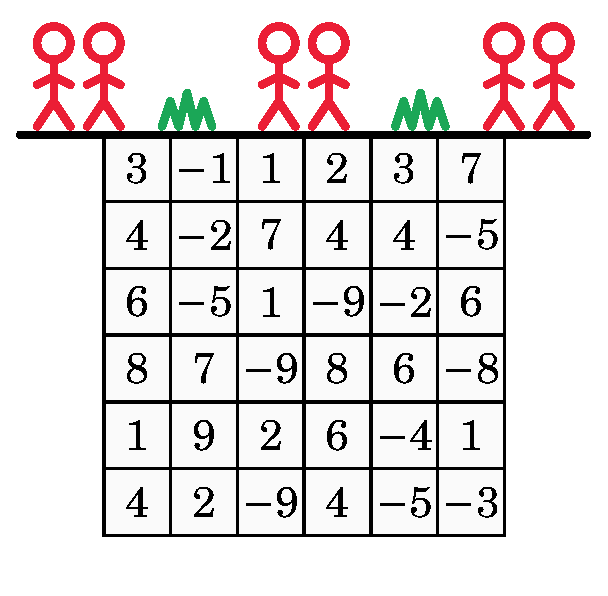
\includegraphics[scale=0.6]{figures/coding_descendingdrills_01.eps}
\end{center}

\subsection*{\sectionfont\upshape Drilling Constraints}
เราต้องการจะเจาะผืนดินเพื่อล่าสมบัติที่อยู่ในดินให้ได้ผลรวมมากที่สุด แต่เนื่องด้วยขีดจำกัดของนวัตกรรมการขุดเจาะที่ยังมีราคาแพง ทำให้เรามีโอกาสเดียวเท่านั้นในการขุดเจาะผืนดินดังกล่าว ลักษณะเส้นทางของการขุดดินจะมีเงื่อนไขดังนี้
\begin{itemize}
\item เราสามารถเริ่มต้นขุดเจาะจากผิวดิน เหนือช่องคอลัมน์ใดก็ได้
\item ตลอดการขุดเจาะในครั้งนี้ เราสามารถขุดเจาะดินในแนวดิ่ง 
    เผื่อลงไปยังชั้นดินชั้นต่อไปก็ได้ หรือจะขุดเจาะในแนวราบไปทางซ้ายหรือขวาในชั้นดินระดับเดียวกันก็ได้ 
    แต่ไม่สามารถเจาะสวนทางแรงโน้มถ่วงในทิศทางชี้สู่ผิวดินได้
\item สำหรับการขุดเจาะแนวราบนั้น เมื่อเราขุดเจาะลงสู่ชั้นดินหนึ่ง ๆ 
    เครื่องขุดเจาะอาจจะเลือกขุดเจาะไปทางซ้ายหรือทางขวา ทิศทางใดทิศทางหนึ่งเท่านั้น 
    (หรือจะไม่ขยับในแนวราบก็ได้) และการขุดแนวราบดังกล่าว จะขยับจากจุดเริ่มต้นได้ไม่เกิน $K$ ช่อง
\item เครื่องขุดเจาะไม่สามารถเดินถอยหลังไปยังช่องดินที่เคยขุดเจาะไปแล้วได้ ไม่ว่าจะเป็นแนวดิ่งหรือแนวราบก็ตาม
\item การขุดเจาะจะสิ้นสุดที่ช่องใดก็ได้\;
    และมูลค่ารวมของสมบัติที่เก็บสะสมได้ คือผลรวมของมูลค่าของสมบัติทุกช่องที่เครื่องขุดเจาะนี้แทรกผ่าน

\item ไม่จำเป็นว่าจะต้องขุดเจาะถึงชั้นผิวดินแถวล่างสุดเสมอไป
\item สมบัติที่มีมูลค่าติดลบที่ค้นพบระหว่างทางจะต้องถูกนำมารวมในผลรวมด้วยเสมอ
\item หากไม่มีรูปแบบการขุดเจาะที่ทำให้ผลรวมสมบัติเป็นบวกเลย สามารถตอบ \verb|0| ได้
\end{itemize}

\bigskip\noindent
\textbf{\uline{ตัวอย่าง}} รูปต่อไปนี้มีเส้นสีส้มแสดงเส้นทางการขุดเจาะชั้นดิน เพื่อล่าสมบัติที่อยู่ในดิน\;
โดยมีเงื่อนไขว่า $K=2$ สังเกตว่าไม่มีการขยับในแนวราบเกิน 2 ช่องเลยในทุกระดับชั้นดิน

ผลรวมมูลค่าสมบัติที่ขุดเจาะตามเส้นทางตัวอย่างนี้คือ 63 หน่วย ซึ่งเป็นเส้นทางที่ดีที่สุดสำหรับรูปตัวอย่างนี้
\begin{center}
    \vspace*{-1.5\baselineskip}
    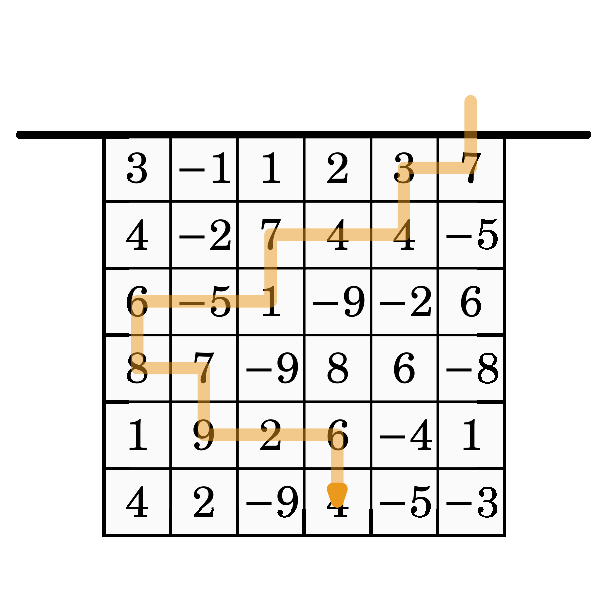
\includegraphics[scale=0.6]{figures/coding_descendingdrills_02.eps}
\end{center}

\subsection*{\sectionfont\upshape Problem Statement}

กำหนดให้มูลค่าของสมบัติในดินเป็นตารางสี่เหลี่ยมผืนผ้าขนาด $R$ แถวและ $C$ คอลัมน์ 
จงหามูลค่าสมบัติรวมที่มากที่สุดที่เกิดจากการขุดเจาะด้วยโอกาสเพียง 1 ครั้งตามเงื่อนไขข้างต้น

\subsection*{\sectionfont\upshape Program Specification}

โปรแกรมที่คุณเขียนจะต้องอ่านข้อมูลจาก stardard input 
และเขียนคำตอบลง standard output โดยข้อมูลจะมีฟอร์แมตดังต่อไปนี้

\bigskip\noindent
{\sectionfont\bfseries Input Format}
\begin{itemize}
\item บรรทัดที่ 1: มีจำนวนเต็มสามตัว $R, C, K$ คั่นด้วยช่องว่าง
\item อีก $R$ บรรทัดถัดมา บรรทัดที่ $i+1$ จะมีจำนวนเต็ม $C$ จำนวน คั่นด้วยช่องว่าง แทนมูลค่าของสมบัติในชั้นดินที่ $i$ เรียงจากซ้ายไปขวา
\begin{lstlisting}
R C K
v[1, 1] v[1, 2] ... v[1, C]
v[2, 1] v[2, 2] ... v[2, C] <%\SuppressNumber\AlternateNumber{...}%>
                            <%\AlternateNumber{R+1}%>
v[R, 1] v[R, 2] ... v[R, C] <%\ReactivateNumber%>
\end{lstlisting}
\end{itemize}

\medskip\noindent
{\sectionfont\bfseries Output Format}
\begin{itemize}
\item คำตอบประกอบด้วยจำนวนเต็มเพียงหนึ่งตัว 
    ซึ่งระบุผลรวมของสมบัติที่มากที่สุดที่สามารถหาได้จากการขุดเจาะเพียงครั้งเดียวตามเงื่อนไขที่กำหนดไว้
\end{itemize}

\newpage
\subsection*{\sectionfont\upshape Data Examples}
\begin{tabular}{p{0.45\linewidth}p{0.45\linewidth}}
\toprule
Example Input & Example Output \\
\midrule
\ttfamily\setstretch{0.8}
6 6 2 \newline
3 -1 1 2 3 7 \newline
4 -2 7 4 4 -5 \newline
6 -5 1 -9 -2 6 \newline
8 7 -9 8 6 -8 \newline
1 9 2 6 -4 1 \newline
4 2 -9 4 -5 -3 &
\ttfamily\setstretch{0.8} 63 \\
\midrule
\ttfamily\setstretch{0.8}
6 5 1 \newline
-1 -1 -1 -1 -1 \newline
-1 1 1 -1 -1 \newline
-1 -1 -1 -1 -1 \newline
-1 -1 1 1 -1 \newline
-2 -2 -2 -2 -2 \newline
-1 1 -1 1 0 &
\ttfamily\setstretch{0.8} 2 \\
\bottomrule
\end{tabular}

\medskip\noindent
\textbf{อธิบายตัวอย่างที่ 2:} โปรดพิจารณารูปตัวอย่างต่อไปนี้ประกอบข้อมูลตัวอย่างข้างต้น 

\begin{center}
    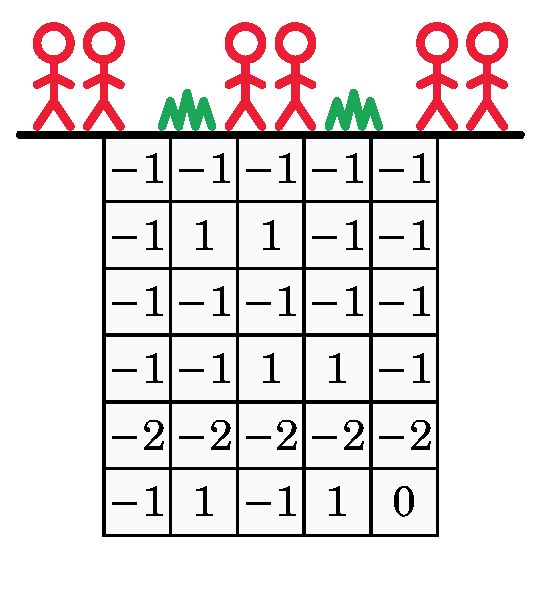
\includegraphics[scale=0.6]{figures/coding_descendingdrills_03.eps}
    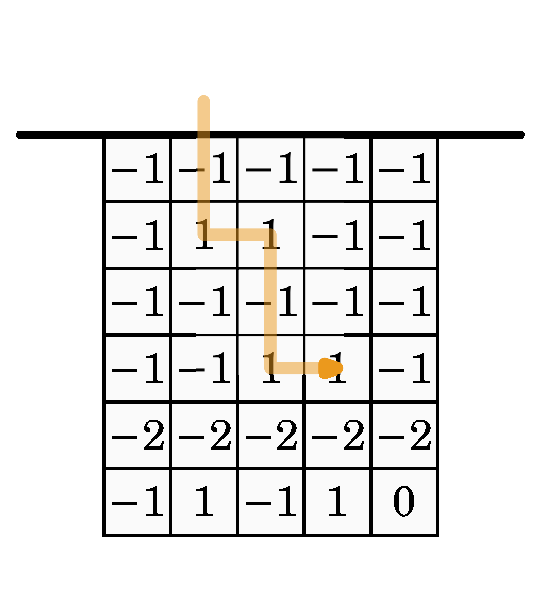
\includegraphics[scale=0.6]{figures/coding_descendingdrills_04.eps}
\end{center}

\subsection*{\sectionfont\upshape Constraints}

โปรแกรมของคุณจะถูกทดสอบกับ test cases สองชุด (เรียกว่าชุดเล็ก และชุดใหญ่)
\begin{itemize}
\item test cases ชุดเล็กจะมีเงื่อนไขว่า 
    ขนาดของตารางจะสอดคล้องกับเงื่อนไขที่ว่า \\ $1 \leq R, C \leq 200$
\item test cases ชุดใหญ่จะมีเงื่อนไขว่า 
    จำนวนช่องในตารางจะสอดคล้องกับเงื่อนไขที่ว่า \\ $1 \leq RC \leq 2 \cdot 10^6$
\item สำหรับทุก test cases จะมีเงื่อนไขว่า 
    จำนวนช่องที่ขยับได้ในแนวราบในแถว ๆ หนึ่งจะสอดคล้องกับเงื่อนไข $0 \leq K < C$ 
    และมูลค่าสมบัติแต่ละช่องจะมีค่าที่สอดคล้องกับเงื่อนไข 
    $-1000 \leq \text{\ttfamily v[i, j]} \leq 1000$
\end{itemize}

\newpage
\question{\bfseries Polymer Chain}

\subsection*{\sectionfont\upshape Background}

ในห้องปฏิบัติการวิจัยเคมีแห่งหนึ่ง มีการทดลอง Simulation การเปลี่ยนแปลงโครงสร้างสาย polymer 
ชื่อ polymer $K$ ซึ่งประกอบไปด้วยอะตอมหลากหลายชนิดเรียงตัวเป็นเส้นตรง

ในคอมพิวเตอร์ เราจะแทนอะตอมแต่ละชนิดด้วยอักขระ \verb|"A"| ถึง \verb|"Z"| 
และเราจะแทน polymer \lstinline{K} ที่มีความยาว $N$ ด้วยสตริงที่ประกอบไปด้วยอักขระ 
\verb|"A"| ถึง \verb|"Z"| ความยาว $N$ ตัว

ในห้องปฏิบัติการดังกล่าว ยังมีเครื่องจัดเรียง polymer ที่มีชื่อว่า
\begin{center}
    \lstinline{manipulate_polymer_once(K[0...N-1], p)} 
\end{center} 
ซึ่งมี Specification ในการทำงานดังต่อไปนี้

\begin{fullwidth}
    \vspace{2\baselineskip}
    \begin{quote}
        หาก input string \lstinline{K} ของฟังก์ชัน \lstinline{manipulate_polymer_once}
        คือลำดับของอักขระ \verb|K[0]|, \verb|K[1]|, \ldots, \verb|K[N-1]| ตามลำดับ 
        และ \lstinline{p} คือ index ของสตริง \lstinline{K} โดยที่ \lstinline{0 <= p <= N-1} 
        แล้ว ฟังก์ชันนี้จะ return ค่าสตริงซึ่งประกอบด้วยอักขระต่อไปนี้ตามลำดับ
        \[
            \underbrace{\text{\ttfamily K[p-1], K[p-2], \ldots, K[1], K[0],}}_\text{exists if $p > 0$}
            \text{\ttfamily K[p],} 
            \underbrace{\text{\ttfamily K[N-1], K[N-2], \ldots, K[p+2], K[p+1]}}_\text{exists if $p < N-1$}
        \]    
        ยกตัวอย่างเช่น ถ้า input ของ \lstinline{manipulate_polymer_once} ได้แก่ 
        \lstinline{K = "ASDFGHJKL"} และ \lstinline{p = 3}\;
        จะได้ output string เป็น \lstinline{"DSAFLKJHG"}\;
        สังเกตว่า \verb|F| จะอยู่ในตำแหน่งเดิมไม่เปลี่ยนแปลง แต่สตริงย่อยที่อยู่ข้างหน้าและข้างหลังจะถูกเรียงกลับหลัง
    \end{quote}
    \vspace{2\baselineskip}
\end{fullwidth}

ในการทำการทดลอง Simulation จริง เราจะนำ polymer สายหนึ่งมาจัดเรียงใหม่ไปเรื่อย ๆ 
อย่างต่อเนื่องเป็นจำนวน $M$ ครั้ง โดยปรับเปลี่ยน parameter ไปเรื่อย ๆ เช่น ถ้า polymer ตั้งต้นคือ 
\lstinline{K = "ASDFGHJKL"} และค่า parameter ของการจัดเรียง $M = 3$ ครั้งอย่างต่อเนื่องคือ 
\lstinline{p_1 = 3}, \lstinline{p_2 = 6}, \lstinline{p_3 = 0} เราจะได้ Polymer ผลลัพธ์เป็น
\begin{center}
    \texttt{ASDFGHJKL → DSAFLKJHG → KLFASDJGH → KHGJDSAFL}
\end{center}

\subsection*{\sectionfont\upshape Problem Statement}

จงเขียนโปรแกรมเพื่อทำ Simulation ของการจัดเรียง polymer สายหนึ่งด้วยลำดับของพารามิเตอร์ที่กำหนดให้ 
แล้วหาว่า polymer ผลลัพธ์สุดท้ายมีหน้าตาเป็นอย่างไร

\newpage
\subsection*{\sectionfont\upshape Program Specification}

โปรแกรมที่คุณเขียนจะต้องอ่านข้อมูลจาก stardard input 
และเขียนคำตอบลง standard output โดยข้อมูลจะมีฟอร์แมตดังต่อไปนี้

\bigskip\noindent
{\sectionfont\bfseries Input Format}
\begin{itemize}
\item บรรทัดที่ 1: มีจำนวนเต็มสองจำนวน $N$ และ $M$ คั่นด้วยช่องว่าง
\item บรรทัดที่ 2: มีสตริงความยาว $N$ ซึ่งระบุข้อมูลสาย Polymer เริ่มต้นก่อนการทดลอง
\item อีก $M$ บรรทัดถัดมา บรรทัดที่ $i+2$ จะมีค่า $p_i$ ซึ่งเป็น Parameter ของคำสั่งการจัดเรียง Polymer คำสั่งที่ $i$ ที่ต้องกระทำดับ Polymer $K$ ตามลำดับ
\begin{lstlisting}
N M
K[0...N-1]
p_1
p_2 <%\SuppressNumber\AlternateNumber{...}%>
    <%\AlternateNumber{M+2}%>
p_M <%\ReactivateNumber%>
\end{lstlisting}
\end{itemize}

\medskip\noindent
{\sectionfont\bfseries Output Format}\begin{itemize}
\item คำตอบประกอบตัวสตริง 1 ตัว ซึ่งก็คือสาย Polymer สุดท้ายหลังจากจัดเรียง Polymer ตามคำสั่งทั้งหมด $M$ ตามที่กำหนดให้ใน input
\end{itemize}

\subsection*{\sectionfont\upshape Data Example}
\begin{tabular}{p{0.45\linewidth}p{0.45\linewidth}}
\toprule
Example Input & Example Output \\
\midrule
\ttfamily\setstretch{0.8}
9 3 \newline
ASDFGHJKL \newline
3 \newline
6 \newline
0 &
\ttfamily\setstretch{0.8} KHGJDSAFL \\
\bottomrule
\end{tabular}

\subsection*{\sectionfont\upshape Constraints}

โปรแกรมของคุณจะถูกทดสอบกับ test cases สองชุด (เรียกว่าชุดเล็ก และชุดใหญ่)
\begin{itemize}
\item test cases ชุดเล็กจะมีเงื่อนไขว่า ความยาว polymer จะสอดคล้องกับเงื่อนไข \\
    $1 \leq N \leq 300$ 
    และจำนวนครั้งที่เรียกใช้งานเครื่องจัดเรียง polymer 
    สอดคล้องกับเงื่อนไข $0 \leq M \leq 30,\!000$
\item test cases ชุดใหญ่จะมีเงื่อนไขว่า ความยาว polymer จะสอดคล้องกับเงื่อนไข \\
    $1 \leq N \leq 300,\!000$ 
    และจำนวนครั้งที่เรียกใช้งานเครื่องจัดเรียง polymer 
    สอดคล้องกับเงื่อนไข $0 \leq M \leq 300,\!000$
\end{itemize}

\newpage
\question{\bfseries Lobbying Tollway}

\subsection*{\sectionfont\upshape Background}

บริษัทขนส่งสินค้าแห่งหนึ่ง จำเป็นต้องวางแผนการลำเลียงส่งสินค้าระหว่างเมืองสองเมืองในดินแดนที่มีเมืองทั้งสิ้น $N$ เมือง 
และมีโครงข่ายของถนน $M$ สายที่เชื่อมเมืองเหล่านี้ให้เดินทางไปมาหาสู่กันได้ทั้งหมด 
เมืองแต่ละเมืองจะมีหมายเลข $1$ ถึง $N$ ส่วนถนนแต่ละสายจะมีหมายเลข $1$ ถึง $M$ ตามลำดับ

สำหรับแต่ละ $i=1,2,\ldots,M$ ถนนสายที่ $i$ จะเป็นถนนวิ่งทางเดียว (one-way road) 
ที่เชื่อมการเดินทางจากเมือง $u_i$ ไปยังเมือง $v_i$ เสมอ ($1 \leq u_i, v_i \leq N$) 
นอกจากนั้นอาจจะมีค่าผ่านทาง $p_i$ บาทที่คนใช้ถนนสายนี้ต้องจ่ายเพื่อใช้งาน ($p_i \geq 0$) 
นอกจากนั้น กำหนดว่าถ้าถนนสายไหนไม่มีค่าผ่านทาง นั่นแปลว่า $p_i = 0$

พึงทราบว่า อาจมีถนนวิ่งทางเดียวที่เชื่อมจากเมืองหนึ่งไปยังอีกเมืองหนึ่ง มากกว่า 1 สายก็ได้ 
นอกจากนั้นอาจมีถนนที่เชื่อมระหว่างเมืองสองเมือง ไป-กลับ โดยที่ถนนเหล่านี้เก็บค่าผ่านทางที่ไม่เท่ากันก็ได้

โดยปกตินั้น บริษัทนี้ได้สำรวจเส้นทางทั้งหมดที่เป็นไปได้ เพื่อใช้ลำเลียงสินค้าจากเมืองหมายเลข $1$ ไปยังเมืองหมายเลข $N$ 
โดยเส้นทางเหล่านี้ล้วนแต่เป็นเส้นทางที่เสียค่าผ่านทางรวมน้อยที่สุดทั้งสิ้น

ในเวลาต่อมา บริษัทนี้ต้องการเปิดเส้นทางการลำเลียงสินค้าเพิ่มขึ้นอย่างน้อย 1 เส้นทาง โดยมีเงื่อนไขต่อไปนี้
\begin{itemize}
\item บริษัทจะไปล็อบบี้กับผู้บริหารของเครือข่ายถนน เพื่อให้ลดค่าผ่านทางของถนนเพียง 1 สายเท่านั้น
\item ค่าผ่านทางใหม่นั้นจะติดลบไม่ได้
\item ค่าผ่านทางใหม่นั้นจะต้องลดลงจากค่าผ่านทางเดิม เป็นปริมาณเงินน้อยที่สุดเท่าที่เป็นไปได้
\item เส้นทางการลำเลียงสินค้าเดิมที่เคยสำรวจไว้จะต้องไม่กระทบ กล่าวคือเส้นทางเดิมแต่ละเส้นทางจะยังคงใช้งานได้เช่นเดิม และมีค่าผ่านทางรวมเท่าเดิม ไม่เพิ่มขึ้นหรือลดลง
\item จะต้องมีเส้นทางใหม่การลำเลียงสินค้าเกิดขึ้นอย่างน้อย 1 เส้นทาง และจะต้องไม่ซ้ำกันเส้นทางเดิมที่บริษัทเคยสำรวจไว้ และราคาค่าผ่านทางรวมของเส้นทางใหม่นี้จะต้องเท่ากับราคาค่าผ่านทางรวมของเส้นทางเดิมอื่น ๆ ของบริษัทด้วย
\end{itemize}

\subsection*{\sectionfont\upshape Problem Statement}

จงรับข้อมูลเครือข่ายถนนในดินแดนแห่งหนึ่ง รวมถึงค่าผ่านทางของถนนแต่ละสาย 
แล้วหาว่าบริษัทนี้จะต้องไปล็อบบี้เพื่อลดค่าผ่านทางของถนนสายใด 1 สาย 
และเป็นปริมาณเงินลดลงน้อยที่สุดเท่าใด จึงจะสามารถเปิดเส้นทางใหม่เพื่อใช้ลำเลียงสินค้าจากเมือง $1$ ไปเมือง $N$ ได้ 
โดยเส้นทางใหม่ที่เกิดขึ้นนี้จะมีค่าผ่านทางรวมถูกที่สุด และถูกเท่า~ๆ กับเส้นทางอื่น~ๆ ที่เคยมีการสำรวจมาก่อนหน้านี้แล้ว

หากมีถนนที่เป็นไปได้หลายสายที่สามารถล็อบบี้ให้ลดราคาลงเป็นปริมาณที่น้อยที่สุดได้ 
ให้ตอบหมายเลขของถนนทุกสายด้วย

\subsection*{\sectionfont\upshape Program Specification}

โปรแกรมที่คุณเขียนจะต้องอ่านข้อมูลจาก stardard input 
และเขียนคำตอบลง standard output โดยข้อมูลจะมีฟอร์แมตดังต่อไปนี้

\bigskip\noindent
{\sectionfont\bfseries Input Format}
\begin{itemize}
\item บรรทัดที่ 1: มีจำนวนเต็มสองจำนวน $N$ และ $M$ คั่นด้วยช่องว่าง
\item อีก $M$ บรรทัดถัดมา บรรทัดที่ $i+1$: จะมีจำนวนเต็มสามจำนวน $u_i, v_i, p_i$
    (คั่นด้วยช่องว่าง) ระบบข้อมูลของถนนหมายเลข $i$ ซึ่งเป็นถนนวิ่งทางเดียวจากเมืองหมายเลข $u_i$ 
    ไปยังเมืองหมายเลข $v_i$ และเก็บค่าผ่านทาง $p_i$ บาท
\begin{lstlisting}
N M
u_1 v_1 p_1
u_2 v_2 p_2 <%\SuppressNumber\AlternateNumber{...}%>
            <%\AlternateNumber{M+1}%>
u_M v_M p_M <%\ReactivateNumber%>
\end{lstlisting}
\textbf{หมายเหตุ:} ข้อมูล Input จะรับประกันว่า 
มีเส้นทางที่เชื่อมจากเมืองหมายเลข $1$ ไปเมืองหมายเลข $N$ เสมอ
\end{itemize}

\medskip\noindent
{\sectionfont\bfseries Output Format}
\begin{itemize}
\item บรรทัดที่ 1: จะต้องเขียนจำนวนเต็มสองจำนวน $D$ และ $K$ คั่นด้วยช่องว่างหนึ่งช่อง 
    โดยที่ $D$ จะระบุปริมาณค่าผ่านทางที่ลดลงน้อยที่สุดที่เป็นไปได้ และ $K$ คือจำนวนถนนทั้งหมดที่สามารถล็อบบี้ให้ลดค่าผ่านทางได้
\item อีก $K$ บรรทัดถัดมา แต่ละบรรทัดจะมีจำนวนเต็ม 1 จำนวน
    ซึ่งแต่ละจำนวนจะระบุหมายเลขถนนที่สามารถล็อบบี้ได้ นอกจากนั้น หมายเลขถนนทั้งหมดจะต้องเรียงจากน้อยไปมาก

    \textbf{หมายเหตุ:} ในกรณีที่บริษัทไม่สามารถใช้วิธีล็อบบี้ใด ๆ เพื่อเปิดเส้นทางใหม่ได้เลย 
    ให้ตอบว่า $D=0$ และ $K=0$ เป็นกรณีพิเศษ
\end{itemize}

\subsection*{\sectionfont\upshape First Data Example}
\begin{tabular}{p{0.45\linewidth}p{0.45\linewidth}}
\toprule
Example Input & Example Output \\
\midrule
\ttfamily\setstretch{0.8}
7 10 \newline
1 2 8 \newline
1 3 6 \newline
1 4 6 \newline
1 5 3 \newline
1 6 12 \newline
2 7 8 \newline
3 7 5 \newline
4 7 7 \newline
5 7 8 \newline
6 7 1 &
\ttfamily\setstretch{0.8}
2 3 \newline
3 \newline
5 \newline
8 \\
\bottomrule
\end{tabular}

\newpage\noindent
\textbf{อธิบายตัวอย่างที่ 1:} 
\begin{itemize}
\item จากตัวอย่างข้อมูลนี้ พบว่าจะมีเส้นทางลำเลียงที่ใช้ค่าผ่านทางรวมน้อยที่สุด 11 บาท 
    ซึ่งมี 2 เส้นทาง ได้แก่ (1) เส้นทางที่ใช้ถนนหมายเลข $2 \,\&\, 7$ 
    และอีกเส้นทางที่ใช้ถนนหมายเลข $4 \,\&\, 9$
\item หากเราล็อบบี้ให้มีการลดค่าผ่านทาง 2 บาท ให้แก่ถนน 1 สายในบรรดาถนน 3 สาย 
    สายได้ก็ได้ (ซึ่งได้แก่ถนนหมายเลข $3$, $5$ และ $8$) 
    แล้วจะทำให้มีเส้นทางลำเลียงสินค้าเส้นทางใหม่ที่ใช้เงินรวม 11 บาทเช่นกัน
\end{itemize}

\subsection*{\sectionfont\upshape Second Data Example}
\begin{tabular}{p{0.45\linewidth}p{0.45\linewidth}}
\toprule
Example Input & Example Output \\    
\midrule
\ttfamily\setstretch{0.8}
4 5 \newline
1 2 2 \newline
1 3 3 \newline
2 3 1 \newline
2 4 3 \newline
3 4 2 &
\ttfamily\setstretch{0.8} 
0 0 \\
\bottomrule
\end{tabular}

\subsection*{\sectionfont\upshape Constraints}

โปรแกรมของคุณจะถูกทดสอบกับ test cases สองชุด (เรียกว่าชุดเล็ก และชุดใหญ่)
\begin{itemize}
\item test cases ชุดเล็กจะมีเงื่อนไขว่า จำนวนเมืองทั้งหมดจะสอดคล้องกับเงื่อนไข \\
    $3 \leq N \leq 50$ และจำนวนถนนทั้งหมดจะสอดคล้องกับเงื่อนไข $1 \leq M \leq 2,\!000$
\item test cases ชุดใหญ่จะมีเงื่อนไขว่า จำนวนเมืองทั้งหมดจะสอดคล้องกับเงื่อนไข \\
    $3 \leq N \leq 100,\!000$ และจำนวนถนนทั้งหมดจะสอดคล้องกับเงื่อนไข $1 \leq M \leq 200,\!000$
\item สำหรับทุก test cases จะมีเงื่อนไขว่า ค่าผ่านทางเริ่มต้นของถนนทุกสายจะสอดคล้องกับเงื่อนไข 
    $0 \leq p_i \leq 5,\!000$
\end{itemize}

\newpage
\question{\bfseries Intercept Meteor}

\subsection*{\sectionfont\upshape Background}

องค์การบริหารการบินและอวกาศแห่งโลกได้ตรวจพบอุกกาบาตขนาดใหญ่ที่กำลังพุ่งชนโลก 
จึงได้เตรียมแผนการรับมือโดยการส่งนักขุดเจาะฝีมือดีขึ้นไปวางระเบิดที่แกนของอุกกาบาตเพื่อระเบิดอุกกาบาตออกเป็นชิ้นเล็ก ๆ 
ก่อนจะตกลงสู่พื้นโลก จากการคาดการณ์ เศษอุกกาบาตส่วนใหญ่จะตกลงสู่ทะเล 
มีเพียงเกาะโคะเกาะเดียวเท่านั้นที่มีคนอาศัยอยู่และได้รับผลกระทบจากเศษอุกกาบาต

เพื่อปกป้องเกาะโคะที่มีอารยธรรมโบราณอันมีคุณค่า 
องค์การบริหารการบินและอวกาศแห่งโลกจึงได้ติดตั้งฐานยิงจรวดมิสไซล์ไว้ที่เกาะโคะเพื่อยิงเศษอุกกาบาตก่อนจะตกถึงพื้น
ข้อเสียของการใช้จรวดมิสไซล์คือ การยิงเศษอุกกาบาตแต่ละครั้งจะสร้างมลพิษสู่ชั้นบรรยากาศเป็นจำนวนมาก
องค์การบริหารการบินและอวกาศแห่งโลกจึงต้องการยิงเศษอุกกาบาตให้น้อยที่สุด
โดยจะยิงเฉพาะเศษอุกกาบาตที่มีจุดตกอยู่บนพื้นเกาะโคะเท่านั้น

ความพิเศษของเกาะโคะคือมีลักษณะเป็น convex polygon 
(เป็นรูปหลายเหลี่ยม และทุกคู่จุดใด ๆ บนเกาะสามารถเดินเป็นเส้นตรงถึงกันได้โดยไม่มีทะเลมาขวาง)

\subsection*{\sectionfont\upshape Problem Statement}

องค์การบริหารการบินและอวกาศแห่งโลกต้องการให้คุณเขียนโปรแกรมช่วยคำนวนว่าจากจุดตกของเศษอุกกาบาตแต่ละลูก 
มีลูกไหนตกบนพื้นเกาะโคะ, ตกตรงขอบเกาะโคะ และ ตกนอกเกาะโคะบ้าง

ให้พิจารณาเฉพาะ\uline{จุด}ตกเท่านั้น ไม่ต้องสนใจขนาดของเศษอุกกาบาต

\subsection*{\sectionfont\upshape Program Specification}

โปรแกรมที่คุณเขียนจะต้องอ่านข้อมูลจาก stardard input 
และเขียนคำตอบลง standard output โดยข้อมูลจะมีฟอร์แมตดังต่อไปนี้

\bigskip\noindent
{\sectionfont\bfseries Input Format}
\begin{itemize}
\item บรรทัดแรก เป็นจำนวนเต็มบวก $N$ แทนจำนวนมุมของ convex polygon $C$ ที่แสดงขอบเขตของเกาะโคะ
\item $N$ บรรทัดต่อมา แต่ละบรรทัดเป็นจำนวนเต็ม $x$ $y$ คั่นด้วยช่องว่าง 
    แทนพิกัดจุดมุมแต่ละจุดของ C เรียงตามเข็มนาฬิกา โดยเริ่มจากจุดที่มีค่า $x$ น้อยที่สุด 
    หากมีจุดที่มีค่า $x$ น้อยที่สุดมากกว่าหนึ่งจุดจะเริ่มต้นจากจุดที่มีค่า $y$ น้อยที่สุด 
    (รับประกันว่าไม่มีพิกัดใดซ้ำกันเลย และ ไม่มี 3 จุดมุมใดๆที่เรียงต่อเนื่องกันเป็นเส้นตรง)
\item บรรทัดต่อมา เป็นจำนวนเต็มบวก $K$ แทนจำนวนเศษอุกกาบาตที่ต้องการตรวจสอบ
\item $K$ บรรทัดต่อมา แต่ละบรรทัดเป็นจำนวนเต็ม $x$ $y$ คั่นด้วยช่องว่าง 
    แทนพิกัดของจุดตกของเศษอุกกาบาตที่ต้องการตรวจสอบแต่ละลูก
\end{itemize}

\medskip\noindent
{\sectionfont\bfseries Output Format}
สำหรับเศษอุกกาบาตที่ต้องการตรวจสอบแต่ละลูก ให้แสดงข้อความในหนึ่งบรรทัด โดยข้อความจะเป็น

\newpage
\begin{fullwidth}
    \begin{itemize}[itemsep=0pt]
        \item \lstinline|"Inside"| หากจุดตกอยู่ภายในเกาะโคะ หรือ
        \item \lstinline|"Outside"| หากจุดตกอยู่ภายนอกเกาะโคะ หรือ
        \item \lstinline|"On the boundary"| หากจุดตกอยู่บนเส้นรอบรูปของเกาะโคะพอดี 
        (อยู่บนขอบหรืออยู่ที่จุดมุมก็ได้)
    \end{itemize}
\end{fullwidth}

\subsection*{\sectionfont\upshape Data Example}
\begin{tabular}{p{0.45\linewidth}p{0.45\linewidth}}
\toprule
Example Input & Example Output \\
\midrule
\ttfamily\setstretch{0.8}
7 \newline
-5 1 \newline
0 6 \newline
6 10 \newline
10 11 \newline
10 9 \newline
5 4 \newline
0 2 \newline
6 \newline
0 5 \newline
-4 9 \newline
5 4 \newline
10 10 \newline
10 3 \newline
5 5 &
\ttfamily\setstretch{0.8}
Inside \newline
Outside \newline
On the boundary \newline
On the boundary \newline
Outside \newline
Inside \\
\bottomrule
\end{tabular}

\medskip\noindent
\textbf{อธิบายตัวอย่าง:} รูปล่างของเกาะโคะมีลักษณะดังที่ปรากฏทาง\ifpageodd{ขวา}{ซ้าย}มือ\;
นอกจากนั้นมี 6 คำถามดังต่อไปนี้
\marginnote{
    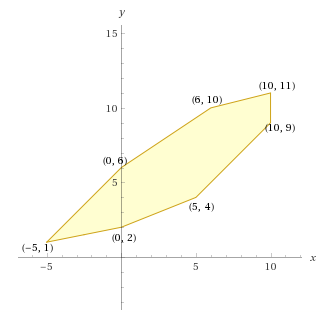
\includegraphics[width=0.96\linewidth]{figures/coding_national_interceptmeteor.png}
}
\begin{itemize}[itemsep=0pt]
\item คำถามแรก จุด (0, 5) อยู่ภายใน C ตอบว่า \lstinline|"Inside"|
\item คำถามที่สอง จุด (-4, 9) อยู่ภายนอก C ตอบว่า \lstinline|"Outside"|
\item คำถามที่สาม จุด (5, 4) เป็นจุดมุม ตอบว่า \lstinline|"On the boundary"|
\item คำถามที่สี่ จุด (10, 10) อยู่บนขอบ ตอบว่า \lstinline|"On the boundary"|
\item คำถามที่ห้า จุด (10, 3) อยู่ภายนอก C ตอบว่า \lstinline|"Outside"|
\item คำถามที่หก จุด (5, 5) อยู่ภายใน C ตอบว่า \lstinline|"Inside"|
\end{itemize}

\subsection*{\sectionfont\upshape Constraints}

โปรแกรมของคุณจะถูกทดสอบกับ test cases สองชุด (เรียกว่าชุดเล็ก และชุดใหญ่)
\begin{itemize}
\item test cases ชุดเล็กจะมีเงื่อนไขว่า จำนวนมุมของ convex polygon 
    ที่แสดงขอบเขตของเกาะโคะสอดคล้องกับเงื่อนไข $3 \leq N \leq 1,\!000$ 
    และจำนวนเศษอุกกาบาตที่ต้องการตรวจสอบสอดคล้องกับเงื่อนไข $1 \leq K \leq 1,\!000$
\item test cases ชุดใหญ่จะมีเงื่อนไขว่า จำนวนมุมของ convex polygon 
    ที่แสดงขอบเขตของเกาะโคะสอดคล้องกับเงื่อนไข $3 \leq N \leq 10^5$ 
    และจำนวนเศษอุกกาบาตที่ต้องการตรวจสอบสอดคล้องกับเงื่อนไข $1 \leq K \leq 10^5$
\item สำหรับทุก test cases จะมีเงื่อนไขว่า พิกัดจุดมุมของ convex polygon 
    ที่แสดงขอบเขตของเกาะโคะ และ พิกัดจุดตกของเศษอุกกาบาตสอดคล้องกับเงื่อนไข \\
    $-10^9 \leq x,y \leq 10^9$
\end{itemize}

\newpage
\question{\bfseries Finding Peep Chan}

\subsection*{\sectionfont\upshape Background}

เด็กหญิงเกดเป็นเด็กน้อยแสนน่ารักที่เลี้ยงแมวเหมียวชื่อว่าปิ๊บจัง วันหนึ่งเจ้าปิ๊บจังหายไปเลยออกไปตามหา 
เด็กหญิงเกดได้เบาะแสมาว่าเจ้าปิ๊บจังไปติดอยู่ในถ้ำแห่งหนึ่ง ถ้ำมีลักษณะเป็น grid 2 มิติ 
แบ่งเป็นห้องขนาด $N \times M$ โดยห้องซ้ายบนสุดคือพิกัด $(1,1)$ และห้องขวาล่างสุดคือพิกัด $(N,M)$

แต่ละห้องจะสามารถเดินไปมาหาสู่กันได้เฉพาะห้องที่ติดกันในทิศทาง บน ล่าง ซ้าย ขวา หรือก็คือ 
ห้อง $(x,y)$ สามารถเดินไปยังห้อง $(x-1,y)$, $(x+1,y)$, $(x,y-1)$ และ $(x,y+1)$ 
นอกจากนี้ในถ้ำยังมีทางลัดอีก $K$ เส้นทาง โดยเส้นทางที่ $i$ 
จะสามารถเดินทางไปมาหาสู่กันระหว่างห้อง $(x_{i1},y_{i1})$ และ $(x_{i2},y_{i2})$ ได้\;
การเดินทางไปยังช่องที่ติดกันในทิศทาง บน ล่าง ซ้าย ขวา หรือ การใช้ทางลัด 
แต่ละครั้งจะใช้เวลาในการเดินทาง 1 วัน (ขอเรียกระยะการเดินของแมวใน 1 วันว่า 1 แมวเดิน)

\begin{center}
    \bigskip
    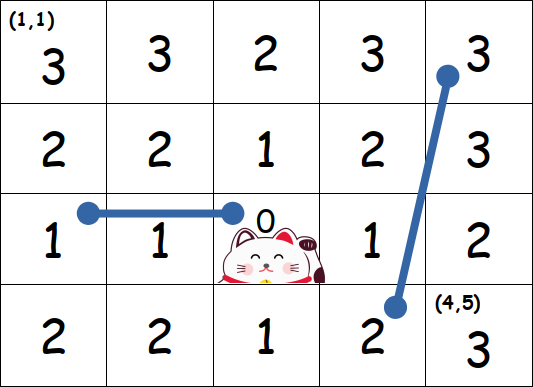
\includegraphics[width=0.7\linewidth]{figures/coding_national_findingpeepchan_01.png}
\end{center}

จากรูปแสดงระยะทางในหน่วยแมวเดิน จากการเดินของแมวที่อยู่ที่ห้องตรงกลาง ลูกศรคือเส้นทางลัด

เด็กหญิงเกดรู้สึกจนปัญญามากเพราะไม่รู้ว่าแมวอยู่ห้องไหนในถ้ำกันแน่ ดังนั้นจะถือว่า \\
\uline{ตอนแรกแมวมีโอกาสที่จะอยู่ในแต่ละห้องด้วยความน่าจะเป็นที่เท่า ๆ กัน} 
(ซึ่งมีค่าเท่ากับ $\frac{1}{N \times M}$) เด็กหญิงเกดจึงไปร้องขอต่อเทพเจ้าให้ช่วยเหลือ

\medskip
เทพเจ้ามีพลังวิเศษ 2 อย่าง คือ
\begin{itemize}
\item \textbf{หยั่งรู้} --- เทพเจ้าจะเลือกห้องห้องหนึ่ง หลังจากนั้นพระเจ้าจะรู้ว่าแมวอยู่ห่างจากห้องที่เลือกเป็น
    ``ระยะทางที่ใกล้ที่สุด'' กี่แมวเดิน แต่ว่าสามารถใช้ได้วันละ 1 ครั้งเท่านั้น
\item \textbf{ช่วยเหลือ} --- เทพเจ้าจะเลือกห้องห้องหนึ่งเพื่อช่วยเหลือแมว 
    ถ้าแมวอยู่ในห้องที่เลือกจะถือว่าช่วยเหลือสำเร็จ แต่ว่าสามารถใช้ได้แค่ครั้งเดียวเท่านั้น
\end{itemize}

เนื่องจากถ้ำมีอากาศอยู่เบาบางมาก แมวจะสามารถมีชีวิตอยู่ได้แค่ 2 วัน 
เพราะฉะนั้นการช่วยเหลือแมวจะมีโอกาสแค่วันนี้กับพรุ่งนี้เท่านั้น

\newpage
เทพเจ้าตอบรับคำร้องขอของเด็กหญิงเกด และดำเนินการช่วยเหลือตามขั้นตอนต่อไปนี้
\begin{enumerate}
\item เทพเจ้าจะใช้พลัง \textbf{“หยั่งรู้”} เพื่อเลือกห้องห้องหนึ่งในถ้ำ
\item เทพเจ้าจะพิจารณาว่า จะใช้พลัง \textbf{“ช่วยเหลือ”} ในวันนี้เลยหรือไม่ 
    แน่นอนว่าถ้าใช้แล้วจะไม่สามารถดำเนินการในข้อต่อไปได้ 
    เพราะไม่สามารถใช้พลัง \textbf{“ช่วยเหลือ”} ได้อีกต่อไป
\item ในกรณีที่เทพเจ้าไม่ได้ใช้พลัง \textbf{“ช่วยเหลือ”} เทพเจ้าจะนอน 1 วันเพื่อพักผ่อน 
    ในขณะที่เทพเจ้านอนพัก แมวจะเคลื่อนที่ 1 ครั้ง 
    โดยการเคลื่อนที่นี้แมวจะสามารถเดินไปยังห้องที่ติดกันหรือห้องที่มีทางลัดไปหากันได้ 
    โดย\uline{แมวจะเดินไปยังห้องที่ไปได้ทั้งหมดด้วย} \uline{โอกาสที่เท่าๆกัน}
\item ในวันถัดไป เทพเจ้าก็จะใช้พลัง \textbf{“หยั่งรู้”} อีกครั้ง
\item เทพเจ้าก็จะใช้พลัง \textbf{“ช่วยเหลือ”} เพราะว่าเป็นโอกาสสุดท้ายที่จะช่วยเหลือแมวแล้ว
\end{enumerate}

\subsection*{\sectionfont\upshape Problem Statement}

เทพเจ้าอยากทราบว่า ความน่าจะเป็นที่มากที่สุดที่เป็นไปได้ที่จะช่วยเหลือแมวได้สำเร็จเป็นเท่าไหร่ 
ถ้าดำเนินการช่วยเหลืออย่าง optimal ที่สุด

\subsection*{\sectionfont\upshape Program Specification}

โปรแกรมที่คุณเขียนจะต้องอ่านข้อมูลจาก stardard input 
และเขียนคำตอบลง standard output โดยข้อมูลจะมีฟอร์แมตดังต่อไปนี้

\bigskip\noindent
{\sectionfont\bfseries Input Format}
\begin{itemize}
\item บรรทัดแรกประกอบด้วยจำนวนเต็ม $N, M$ แทนขนาดของถ้ำ และ K แทนจำนวนเส้นทางลัด
\item K บรรทัดถัดมา บรรทัดที่ $i$ จะประกอบด้วย จำนวนเต็ม 4 จำนวน 
    $x_{i1}$, $y_{i1}$, $x_{i2}$ และ $y_{i2}$ คั่นด้วยช่องว่าง ซึ่งระบุเส้นทางลัดเส้นที่ $i$
\begin{lstlisting}
N M K
x_{1,1} y_{1,1} x_{1,2} y_{1,2}
x_{2,1} y_{2,1} x_{2,2} y_{2,2} <%\SuppressNumber\AlternateNumber{...}%>
                                <%\AlternateNumber{K+1}%>
x_{K,1} y_{K,1} x_{K,2} y_{K,2} <%\ReactivateNumber%>
\end{lstlisting}
\textbf{หมายเหตุ:} รับประกันว่า $1 \leq x_{i1}, x_{i2} \leq N$ และ 
$1 \leq y_{i1},y_{i2} \leq M$ และจะไม่มีเส้นทางลัดซ้ำกัน และไม่มีทางลัดของห้องที่อยู่ติดกัน
\end{itemize}

\medskip\noindent
{\sectionfont\bfseries Output Format}
\begin{itemize}
    \item ตอบเป็นจำนวนจริง 1 จำนวน แทนความน่าจะเป็นที่มากที่สุดที่เป็นไปได้ของการช่วยเหลือแมว
    ถ้าเทพเจ้าทำการช่วยเหลืออย่าง Optimal ที่สุด \\
    (\textbf{หมายเหตุ:} คำตอบจะถูกต้องถ้าคาดเคลื่อนไม่มากกว่าคำตอบจริงเกิน $10^{-6}$)
\end{itemize}

\newpage
\subsection*{\sectionfont\upshape First Data Example}
\begin{tabular}{p{0.45\linewidth}p{0.45\linewidth}}
\toprule
Example Input & Example Output \\
\midrule
\ttfamily\setstretch{0.8}
2 2 1 \newline
1 1 2 2 &
\ttfamily\setstretch{0.8}
0.9166666667 \\
\bottomrule
\end{tabular}

\medskip\noindent
\textbf{อธิบายตัวอย่างที่ 1:} จากตัวอย่างของข้อมูลนำเข้าข้างต้น สามารถแสดงให้เห็นตามรูปที่ปรากฏทางด้านข้าง
โดยที่ลูกศรแสดงเส้นทางลัดระหว่างห้องสองห้อง
\marginnote{%
    \centering
    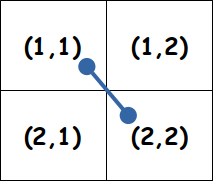
\includegraphics[width=0.7\linewidth]{figures/coding_national_findingpeepchan_02.png}
}

หนึ่งในการวิธีช่วยเหลือที่ optimal ขอเทพเจ้ามีดังต่อไปนี้
\begin{enumerate}
\item วันแรก ใช้พลัง \textbf{“หยั่งรู้”} ที่ห้อง $(1,2)$
    \begin{enumerate}
        \item ความน่าจะเป็น $\frac{1}{4}$ ที่ระยะทางที่ใกล้ที่สุด 
            จะเป็น $0$ แมวจะอยู่ที่ห้อง $(1,2)$ \\
            กรณีนี้สามารถใช้พลัง \textbf{“ช่วยเหลือ”} เพื่อช่วยแมวได้ทันที
        \item ความน่าจะเป็น $\frac{2}{4}$ ที่ระยะทางที่ใกล้ที่สุด 
            จะเป็น 1 แมวอาจจะอยู่ที่ห้อง $(1,1)$ \\
            หรือ $(2,2)$ ก็ได้\; กรณีนี้ควรรอวันที่ 2
        \item ความน่าจะเป็น $\frac{1}{4}$ ที่ระยะทางที่ใกล้ที่สุด 
            จะเป็น 2 แมวจะอยู่ที่ห้อง $(2,1)$ \\
            กรณีนี้สามารถใช้พลัง \textbf{“ช่วยเหลือ”} เพื่อช่วยแมวได้ทันที
    \end{enumerate}
\item จากข้อ 1{\hrsp}(b) ระหว่างวันในขณะที่เทพเจ้านอนพัก การเคลื่อนที่ของแมวเป็นดังนี้
    \begin{itemize}
        \item ความน่าจะเป็นที่แมวจะเดินไปห้อง $(1,2)$ คือ 
            $\frac{2}{4}\times\frac{1}{3}=\frac{2}{12}$ \\ 
            ← เดินจาก $(1,1)$ หรือ $(2,2)$
        \item ความน่าจะเป็นที่แมวจะเดินไปห้อง $(1,1)$ คือ 
            $\frac{1}{4}\times\frac{1}{3}=\frac{1}{12}$ ← เดินจาก $(2,2)$
        \item ความน่าจะเป็นที่แมวจะเดินไปห้อง $(2,2)$ คือ 
            $\frac{1}{4}\times\frac{1}{3}=\frac{1}{12}$ ← เดินจาก $(1,1)$
        \item ความน่าจะเป็นที่แมวจะเดินไปห้อง $(2,1)$ คือ 
            $\frac{2}{4}\times\frac{1}{3}=\frac{1}{12}$ \\
            ← เดินจาก $(1,1)$ หรือ $(2,2)$
    \end{itemize}
\item วันถัดมาวันที่ ใช้พลัง “หยั่งรู้” ที่ห้อง $(1,2)$ เช่นเดิม
    \begin{enumerate}
        \item ความน่าจะเป็น $\frac{2}{12}$ ที่ระยะทางที่ใกล้ที่สุดจะเป็น 0 
            แมวจะอยู่ที่ห้อง $(1,2)$ \\
            กรณีนี้สามารถชใช้พลัง \textbf{“ช่วยเหลือ”} แมวได้แน่นอน
        \item ความน่าจะเป็น $\frac{2}{12}$ ที่ระยะทางที่ใกล้ที่สุดจะเป็น 2 
            แมวจะอยู่ที่ห้อง $(2,1)$ \\
            กรณีนี้สามารถใช้พลัง \textbf{“ช่วยเหลือ”} แมวได้แน่นอน
        \item ความน่าจะเป็น $\frac{1}{12}+\frac{1}{12}=\frac{2}{12}$ 
            ที่ระยะทางที่ใกล้ที่สุดจะเป็น 1 
            แมวจะอาจจะอยู่ที่ห้อง $(1,1)$ หรือ $(2,2)$ ก็ได้ \\
            กรณีนี้ การเลือกห้องใดห้องหนึ่งเพื่อใช้พลัง \textbf{“ช่วยเหลือ”} 
            จะมีโอกาสช่วยแมวสำเร็จด้วยความน่าจะเป็น $\frac{2}{12} \times \frac{1}{2}=\frac{1}{12}$
    \end{enumerate}
\item สรุปว่า ความน่าจะเป็นที่เทพเจ้าจะสามารถช่วยเหลือแมวได้ ตามข้อ 1{\hrsp}(a), 1{\hrsp}(c), 
    3{\hrsp}(a), 3{\hrsp}(b) และ 3{\hrsp}(c) คือ
    \[
        \frac{1}{4} + \frac{1}{4} + \frac{2}{12} + \frac{2}{12} + \frac{1}{12} 
        = \frac{11}{12} \approx 0.9166666667
    \]
\end{enumerate}


\subsection*{\sectionfont\upshape Second Data Example}
\begin{tabular}{p{0.45\linewidth}p{0.45\linewidth}}
\toprule
Example Input & Example Output \\    
\midrule
\ttfamily\setstretch{0.8}
3 3 3 \newline
3 1 1 2 \newline
3 1 2 3 \newline
1 2 3 1 &
\ttfamily\setstretch{0.8} 
0.7259259259 \\
\bottomrule
\end{tabular}

\subsection*{\sectionfont\upshape Constraints}

โปรแกรมของคุณจะถูกทดสอบกับ test cases สองชุด (เรียกว่าชุดเล็ก และชุดใหญ่)
\begin{itemize}
\item test cases ชุดเล็กจะมีเงื่อนไข ขนาดของถ้ำสอดคล้องกับเงื่อนไข 
    $1 \leq N,M \leq 20$ และ $N \times M \leq 200$ 
    และจำนวนเส้นทางลัดสอดคล้องกับเงื่อนไข $1 \leq K \leq 100$
\item test cases ชุดใหญ่จะมีเงื่อนไขว่า ขนาดของถ้ำสอดคล้องกับเงื่อนไข 
    $1 \leq N,M \leq 20$ และจำนวนเส้นทางลัดสอดคล้องกับเงื่อนไข $1 \leq K \leq 70,000$
\end{itemize}

\newpage
\question{\bfseries Stable Molecule}

\subsection*{\sectionfont\upshape Background}

ในห้องปฏิบัติการวิจัยเคมีแห่งหนึ่ง\; คุณกุ้งกำลังศึกษาโครงสร้างของโมเลกุลชนิดหนึ่ง\;
ซึ่งประกอบไปด้วยอะตอมหลากหลายชนิดมาประกอบกันด้วยพันธะที่เชื่อมระหว่างอะตอมบางคู่ จนมีโครงสร้างเป็นกราฟต้นไม้

กล่าวคือโครงสร้างโมเลกุลนี้จะประกอบด้วยอะตอมทั้งสิ้น $N$ ชนิด ชนิดละ 1 อนุภาค (เรียกสั้น ๆ ว่า “ลูก”) 
และมีพันธะทั้งสิ้น $N-1$ พันธะที่เชื่อมอะตอมเหล่านี้เข้าด้วยกัน 
(เราจะเรียกอะตอมแต่ละลูกว่าลูกที่ $i$ สำหรับ $i = 1, 2, \ldots, N$)

คุณกุ้งสามารถกำหนดค่ามวลของอะตอมแต่ละลูกได้ โดยที่มวลของอะตอมลูกที่ $i$ จะกำหนดด้วยตัวแปร $m_i$ 
ซึ่งเป็นจำนวนเต็มบวก กล่าวคือมีเงื่อนไขว่า $m_i \geq 1$

โครงสร้างโมเลกุลนี้จะ \textbf{“เสถียร”} ก็ต่อเมื่อ แรงดึงดูดระหว่างอะตอม 2 ลูกที่เป็นพันธะต่อกันจะมีค่าไม่เกิน $P$ 
โดยแรงดึงดูดระหว่างมวลสามารถคำนวณได้จากผลคูณของมวลของอะตอมแต่ละลูก (นั่นแปลว่า $m_u \times m_v \leq P$ สำหรับทุกคู่อะตอม $u$ และ $v$ ที่มีพันธะต่อกัน)

\bigskip\noindent
\textbf{\uline{ตัวอย่าง}} 
เมื่อพิจารณาโครงสร้างโมเลกุลที่เกิดจากอะตอม 4 ลูกที่เชื่อมกันดังรูปทาง\ifpageodd{ขวา}{ซ้าย} 
และกำหนดให้ $P=12$ แล้วพบว่าโครงสร้างโมเลกุลรูปบนจะเสถียร แต่โครงสร้างอันล่างจะไม่เสถียร
\marginnote[-15\baselineskip]{%
    \centering
    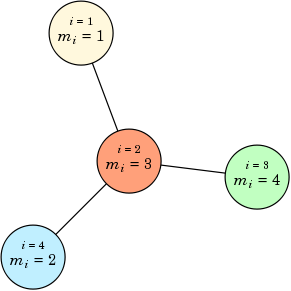
\includegraphics[width=0.97\linewidth]{figures/coding_national_stablemolecule_01.png}

    \bigskip\bigskip
    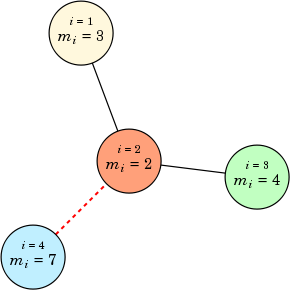
\includegraphics[width=0.97\linewidth]{figures/coding_national_stablemolecule_02.png}
}

\subsection*{\sectionfont\upshape Problem Statement}

จงเขียนโปรแกรมเพื่อรับข้อมูลที่กำหนดโครงสร้างโมเลกุล และค่าขีดจำกัดสูงสุดของแรงดึดดูดระหว่างอะตอม $P$ 
แล้วหาว่าคุณกุ้งจะสามารถกำหนดค่ามวลให้แก่อะตอมแต่ละลูกให้แตกต่างกันได้ทั้งหมดกี่รูปแบบ โดยที่โมเลกุลจะยังเสถียรอยู่

\subsection*{\sectionfont\upshape Program Specification}

โปรแกรมที่คุณเขียนจะต้องอ่านข้อมูลจาก stardard input 
และเขียนคำตอบลง standard output โดยข้อมูลจะมีฟอร์แมตดังต่อไปนี้

\bigskip\noindent
{\sectionfont\bfseries Input Format}
\begin{itemize}
\item บรรทัดที่ 1: มีจำนวนเต็มสองจำนวน $N$ และ $P$ คั่นด้วยช่องว่าง
\item อีก $N-1$ บรรทัดถัดมา บรรทัดที่ $j+1$ จะมีจำนวนเต็ม $u_j$ และ $v_j$ 
    คั่นด้วยช่องว่าง ซึ่งระบุว่ามีพันธะระหว่างอะตอมลูกที่ $u_j$ และอะตอมลูกที่ $v_j$  
\begin{lstlisting}
N P
u_1 v_1
u_2 v_2 <%\SuppressNumber\AlternateNumber{...}%>
        <%\AlternateNumber{N+1}%>
u_N v_N <%\ReactivateNumber%>
\end{lstlisting}
\textbf{หมายเหตุ:} กำหนดให้ $1 \leq u_j, v_j \leq N$ และ $u_j \neq v_j$
\end{itemize}

\medskip\noindent
{\sectionfont\bfseries Output Format}
\begin{itemize}
\item คำตอบประกอบด้วยจำนวนเต็ม 1 ตัว 
    ระบุจำนวนรูปแบบของโมเลกุลที่คุณกุ้งสามารถกำหนดมวลให้อะตอมแต่ละลูกได้ 
    โดยคำตอบจะต้องอยู่ในรูปของเศษที่เกิดจากการหารด้วย $1,\!000,\!000,\!007$
\end{itemize}

\subsection*{\sectionfont\upshape First Data Example}
\begin{tabular}{p{0.45\linewidth}p{0.45\linewidth}}
\toprule
Example Input & Example Output \\
\midrule
\ttfamily\setstretch{0.8}
4 2 \newline
1 2 \newline
2 3 \newline
4 2 &
\ttfamily\setstretch{0.8}
9 \\
\bottomrule
\end{tabular}

\medskip\noindent
\textbf{อธิบายตัวอย่างที่ 1:} เราสามารถแจกแจงรูปแบบของการกำหนดมวลให้อะตอมแต่ละลูกในโมเลกุลได้ดังนี้

\begin{fullwidth}
    \begin{center}
        \bigskip
        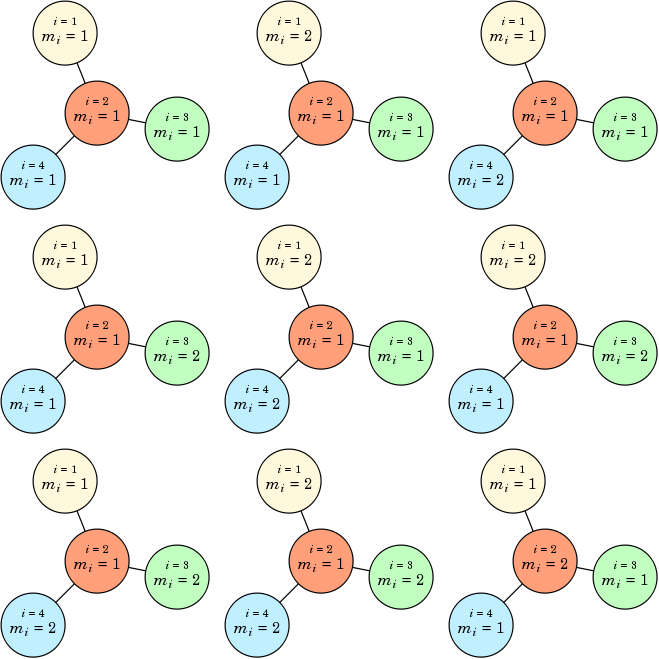
\includegraphics[width=0.9\linewidth]{figures/coding_national_stablemolecule_03.png}
    \end{center}
\end{fullwidth}

\subsection*{\sectionfont\upshape Second Data Example}
\begin{tabular}{p{0.45\linewidth}p{0.45\linewidth}}
\toprule
Example Input & Example Output \\    
\midrule
\ttfamily\setstretch{0.8}
5 3 \newline
4 2 \newline
3 2 \newline
1 3 \newline
5 3 &
\ttfamily\setstretch{0.8} 
51 \\
\bottomrule
\end{tabular}

\subsection*{\sectionfont\upshape Constraints}

โปรแกรมของคุณจะถูกทดสอบกับ test cases สองชุด (เรียกว่าชุดเล็ก และชุดใหญ่)
\begin{itemize}
\item test cases ชุดเล็กจะมีเงื่อนไขว่า ค่าขีดจำกัดสูงสุดของแรงดึดดูดระหว่างอะตอมจะสอดคล้องกับเงื่อนไข $1 \leq P \leq 10^3$
\item test cases ชุดใหญ่จะมีเงื่อนไขว่า ค่าขีดจำกัดสูงสุดของแรงดึดดูดระหว่างอะตอมจะสอดคล้องกับเงื่อนไข $1 \leq P \leq 10^9$
\item สำหรับทุก test cases จะมีเงื่อนไขว่า จำนวนของอะตอมจะสอดคล้องกับเงื่อนไข $1 \leq N \leq 1,\!000$
\end{itemize}

\newpage
\question{\bfseries Rotate Sort (Optimization Problem)}

\begin{quote}
    \em
    \vphantom{~}\llap{\adfdownleafleft\;}โจทย์ Coding
    ข้อนี้ ปรากฏในการแข่งขัน \techjam\ รอบชิงชนะเลิศระดับประเทศ
    โดยเป็นโจทย์ที่ผู้เข้าแข่งขันจะต้อง optimize เพื่อหาคำตอบที่ดีที่สุดในบรรดาผู้เข้าแข่งขันทั้งหมด
    หากโปรแกรมของผู้เข้าแข่งขันให้ผลลัพธ์ที่ดีมากเท่าใด ก็จะยิ่งมีโอกาสได้คะแนนสูงมากขึ้นเท่านั้น

    กติการที่ปรากฏในส่วนของ Submission and Scoring นั้นมีนัยยะสำคัญเฉพาะภายในการแข่งขันดังกล่าวเท่านั้น
    โปรดใช้เนื้อหาดังกล่าวเพื่อการอ้างอิงเท่านั้น
\end{quote}

\subsection*{\sectionfont\upshape Background}

กำหนดให้ operation ชื่อว่า \lstinline|rotate_3way| รับ input argument อยู่ 3 อย่าง ได้แก่
\begin{itemize}
\item array $A$ ของจำนวนเต็ม
\item ดัชนี $p$ และ $q$ ภายใน array $A$ ซึ่ง $1 \leq p \leq q \leq |A|$ \\
    (เมื่อ $|A|$ คือความยาวของ array $A$)
\end{itemize}

เมื่อเรียกใช้งาน \lstinline|rotate_3way(A, p, q)| จะได้ output value เป็น array ที่มีลักษณะเป็นดังนี้
\begin{fullwidth}
    \vspace*{-\baselineskip}
    \[
        \text{\ttfamily rotate\_3way(A, p, q)} =
        \left[
        \underbrace{\text{\ttfamily A[q+1], A[q+2], \ldots, A[N],}}_\text{can be empty}
        \text{\ttfamily A[p], A[p+1],\ldots,A[q],} 
        \underbrace{\text{\ttfamily A[1], A[2], \ldots, A[p-1]}}_\text{can be empty}
        \right]    
    \]    
\end{fullwidth}

\noindent
ยกตัวอย่างเช่น
\begin{itemize}[itemsep=0pt]
\item \lstinline{rotate_3way([5, 2, 1, 0], 2, 3) = [0, 2, 1, 5]}
\item \lstinline{rotate_3way([5, 2, 1, 0], 2, 2) = [1, 0, 2, 5]}
\item \lstinline{rotate_3way([5, 2, 1, 0], 1, 2) = [1, 0, 5, 2]}
\item \lstinline{rotate_3way([5, 2, 1, 0], 1, 4) = [5, 2, 1, 0]}
\end{itemize}

\subsection*{\sectionfont\upshape Problem Statement}

โจทย์ข้อนี้ โปรแกรมของผู้เข้าแข่งขันจะได้รับข้อมูลนำเข้าเป็น array $X$ ของจำนวนเต็มที่ไม่เรียงลำดับ 
กำหนดให้ $N = |X|$ คือความยาวของ array $X$

เป้าหมายของโปรแกรมของผู้เข้าแข่งขันคือ 
จะต้องเรียงลำดับจำนวนใน array $X$ โดยเรียกใช้งาน operation \lstinline|rotate_3way| 
เป็นจำนวนครั้งให้ได้น้อยที่สุดเท่าที่ผู้เข้าแข่งขันสามารถทำได้

กล่าวคือ เมื่อโปรแกรมของผู้เข้าแข่งขันได้รับข้อมูล array $X$ แล้วจะต้องระบุว่าจะเรียกใช้งาน 
\lstinline|rotate_3way| ทั้งสิ้นกี่ครั้ง และในแต่ละครั้ง จะกำหนดค่าดัชนี $p$ และ $q$ เท่าใด
ตามลำดับ

สำหรับเกณฑ์การให้คะแนนในข้อนี้ โปรดดูหัวข้อ Submission and Scoring

\subsection*{\sectionfont\upshape Program Specification}

โปรแกรมที่คุณเขียนจะต้องอ่านข้อมูลจาก stardard input 
และเขียนคำตอบลง standard output โดยข้อมูลจะมีฟอร์แมตดังต่อไปนี้

\bigskip\noindent
{\sectionfont\bfseries Input Format}
\begin{itemize}
\item บรรทัดที่ 1: จะมีจำนวนเต็มหนึ่งจำนวน ระบุ $N$ ซึ่งเป็นความยาวของ array $X$
\item อีก $N$ บรรทัดถัดมา บรรทัดที่ $i+1$ จะระบุจำนวน $X[i]$ ของ array $X$
\begin{lstlisting}
N
X[1]
X[2] <%\SuppressNumber\AlternateNumber{...}%>
     <%\AlternateNumber{N+1}%>
X[N] <%\ReactivateNumber%>
\end{lstlisting}
\end{itemize}

\medskip\noindent
{\sectionfont\bfseries Output Format}
\begin{itemize}
\item บรรทัดที่ 1: จะมีจำนวนเต็ม $K$ หนึ่งจำนวน ระบุจำนวนครั้งที่ operation \lstinline|rotate_3way| 
    จะถูกเรียกใช้งาน
\item อีก $K$ บรรทัดถัดมา บรรทัดที่ $j+1$ จะระบุจำนวนเต็มสองจำนวน $p_j$ และ $q_j$ 
    คั่นด้วยช่องว่ง ซึ่งเป็นดัชนี $p$ และ $q$ ของการเรียกใช้งาน operation \lstinline|rotate_3way| 
    ครั้งที่ $j$
\end{itemize}

\subsection*{\sectionfont\upshape Data Example}
\begin{tabular}{p{0.3\linewidth}p{0.3\linewidth}p{0.3\linewidth}}
\toprule
Example Input & Example Output A & Example Output B \\
\midrule
\ttfamily\setstretch{0.8}
4 \newline
5 \newline
2 \newline
1 \newline
0 &
\ttfamily\setstretch{0.8}
3 \newline
2 2 \newline
2 2 \newline
3 4 &
\ttfamily\setstretch{0.8}
4 \newline
2 4 \newline
2 4 \newline
3 3 \newline
3 3 \\
\bottomrule
\end{tabular}

\medskip\noindent
\textbf{อธิบายตัวอย่าง:} สังเกตว่าลำดับของ operation ที่แสดงในทั้งสองคำตอบข้างต้น 
สามารถทำให้ array  $X$ เรียงลำดับได้ถูกต้อง แต่คำตอบ A ใช้จำนวน operation น้อยกว่า B

\subsection*{\sectionfont\upshape Submission and Scoring}

สำหรับโจทย์ข้อนี้ พึงทราบว่า test case แต่ละอันจะมีคะแนนเต็ม 18 คะแนน นอกจากนั้น 
คะแนนรวมตอนท้ายสำหรับโจทย์ข้อนี้จะคิดจากค่าเฉลี่ยของคะแนนจากแต่ละ test case
จึงทำให้คะแนนรวมสูงสุดที่เป็นไปได้สำหรับข้อนี้คือ 18 คะแนน เช่นกัน 
(เศษทศนิยมของคะแนนจะถูกปัดทิ้งให้เหลือทศนิยม 6 ตำแหน่ง)

\bigskip\noindent
{\sectionfont\bfseries Minimum requirement} \\
สำหรับ test case แต่ละอัน โปรแกรมของผู้เข้าแข่งขันจะถือว่าให้ผลลัพธ์ที่\uline{ถูกต้อง} ก็ต่อเมื่อ
\begin{enumerate}
\item โปรแกรมให้ผลลัพธ์ตรงกับ Program Specification ที่โจทย์กำหนดให้
\item ผลลัพธ์ของโปรแกรมเรียกใช้งาน operation \lstinline|rotate_3way| 
    ที่ทำให้ array $X$ เรียงลำดับจากน้อยไปมากได้ถูกต้อง
\item ผลลัพธ์ของโปรแกรมเรียกใช้งาน operation \lstinline|rotate_3way| ไม่เกิน $100 N$ ครั้ง
\end{enumerate}

\noindent
\textbf{\uline{หมายเหตุ:}} หากโปรแกรมของคุณให้ผลลัพธ์ไม่ถูกต้อง จะได้ 0 คะแนนทันที\newline

\smallskip\noindent
{\sectionfont\bfseries Scoring scheme for correct answers} \\
เมื่อโปรแกรมของคุณให้ผลลัพธ์ที่ถูกต้อง กำหนดให้

\begin{itemize}
\item โปรแกรมของคุณเรียกใช้งาน operation \lstinline|rotate_3way| 
    เป็นจำนวน $K$ ครั้งสำหรับ test case นี้
\item ในบรรดาผู้เข้าแข่งขันทั้งหมด จำนวน operation ที่น้อยที่สุดที่มีผู้เข้าแข่งขันทำได้คือ $K^*$ ครั้ง 
    สำหรับ test case เดียวกัน
\end{itemize}
แล้วคะแนนของคุณสำหรับ test case อันนี้จะคำนวณจากสูตรดังต่อไปนี้
\[
    \begin{cases}
    18 &\quad\text{if $K = K^*$} \\
    6 + 9 \cdot\dfrac{K^*}{K} &\quad\text{if $K > K^*$}
    \end{cases}
\]

สังเกตว่าเมื่อโปรแกรมให้ผลลัพธ์ที่ถูกต้อง รับประกันว่าจะได้คะแนนอย่างน้อย 6 คะแนนสำหรับ test case นั้น ๆ\;
และกำหนดให้เศษที่เกิดขึ้นจากการหาร จะถูกปัดทิ้งให้เหลือทศนิยม 6 ตำแหน่ง

\subsection*{\sectionfont\upshape Constraints}

แต่ละ test case จะมีเงื่อนไขดังต่อไปนี้
\begin{itemize}
\item ความยาวของ array $X$ จะสอดคล้องกับเงื่อนไข $2 \leq N \leq 100$
\item จำนวนที่พบใน array $X$ จะอยู่ในช่วง $0$ ถึง $1000$ ซึ่งอาจมีบางจำนวนซ้ำกันได้
\end{itemize}

